\section{Pump Selection}
% -------------------------------------------------
% 4.1 Pump Selection Criteria
% -------------------------------------------------
\subsection{Pump Selection Criteria}

Pump selection for the proposed lift station is based on the hydraulic requirements established from the system curve analysis developed in the previous chapter. The selected pump must be capable of delivering the required discharge flow while overcoming the calculated \textit{total dynamic head} ($TDH$) of the force main system. The operating point of the pump must therefore occur at the intersection of the pump performance curve and the system curve to ensure that the pump operates within an efficient and stable region of its performance range. This approach follows the pump station design methodology outlined in wastewater lift station design guidance~\cite{ProjectD_Colebrooke_2020}.

Because the station conveys raw municipal wastewater, the pump must be suitable for \textit{non-clog wastewater service} and capable of passing suspended solids commonly present in sanitary sewer systems. In this design, the pump is required to accommodate solids up to approximately $3~\text{in}$ in diameter in order to minimize the risk of clogging and ensure reliable operation under typical wastewater conditions. In addition to meeting the hydraulic head requirement, the pump must also operate efficiently at the selected design flow rate derived from the system curve.

Operational reliability is also an important consideration in wastewater lift station design. Therefore, the pump station is configured with a \textit{duplex pumping arrangement}, where one pump functions as the duty pump and the second pump provides redundancy and assists during higher inflow conditions. This configuration allows continuous operation of the station during maintenance or pump failure and is consistent with common wastewater lift station design practices~\cite{ProjectD_Colebrooke_2020}.


% -------------------------------------------------
% 4.2 Pump Curve Matching
% -------------------------------------------------
\subsection{Pump Curve Matching}

Pump selection is performed by comparing the system curve developed in the previous chapter with the manufacturer's pump performance curves. The system curve represents the relationship between flow rate and the total dynamic head required by the piping system. As flow increases, friction and minor losses increase, resulting in a corresponding increase in the total dynamic head that the pump must overcome. The system curve therefore defines the hydraulic resistance of the force main system.

Pump manufacturers provide pump performance curves that illustrate the relationship between flow rate and head produced by a specific pump model. By plotting the system curve together with the pump performance curve, the operating point of the pump can be identified. The operating point occurs at the intersection of the two curves and represents the flow and head conditions at which the pump will operate within the system.~\cite{Jensen_PumpStationDesignGuidelines_2012}

The pump selected for the proposed lift station must therefore have a performance curve that intersects the system curve near the desired design flow while maintaining acceptable efficiency and stable operation. This procedure ensures that the selected pump can deliver the required flow against the calculated system head while operating within the recommended performance range for wastewater pumping systems~\cite{ProjectD_Colebrooke_2020}.



% -------------------------------------------------
% 4.3 Selected Pump Operating Point
% -------------------------------------------------
\subsection{Selected Pump Operating Point}

The final pump duty point was determined by comparing the system curve developed in Chapter 3 with manufacturer pump performance curves using the Sulzer ABSEL pump selection tool. ABSEL is a web-based hydraulic selection platform developed by Sulzer that allows users to configure application conditions, input the required duty point, and evaluate pump performance curves for water and wastewater applications. The tool enables users to select pumps by defining the operating flow and head requirements and provides outputs including pump curves, hydraulic efficiency, dimensional drawings, and product data sheets. This procedure follows standard pump selection practice in wastewater lift station design where the system curve is compared with manufacturer pump curves to determine the operating point of the pump \cite{Jensen_PumpStationDesignGuidelines_2012,EPA_LiftStation_DesignManual_2004}. The ABSEL tool used for pump selection is provided by Sulzer for water and wastewater pump sizing and hydraulic performance evaluation \cite{Sulzer_ABSEL}.

The design operating point was selected from the system curve developed earlier. At a flow of $120~\text{gpm}$, the calculated system head is $11.8~\text{ft}$. This operating condition satisfies the minimum velocity requirement for wastewater transport within the force main and lies within the hydraulic operating range of the system. The duty point was entered into the Sulzer ABSEL selection tool to identify a pump whose performance curve intersects the system curve near this operating condition. The resulting pump selection corresponds to a Sulzer submersible wastewater pump, model XFP100C VX 1$\sim$ (wet pit installation) equipped with a vortex impeller designed for handling sewage containing suspended solids and fibrous material \cite{Sulzer_PumpCatalog_2024}.


\begin{figure}[H]
\centering
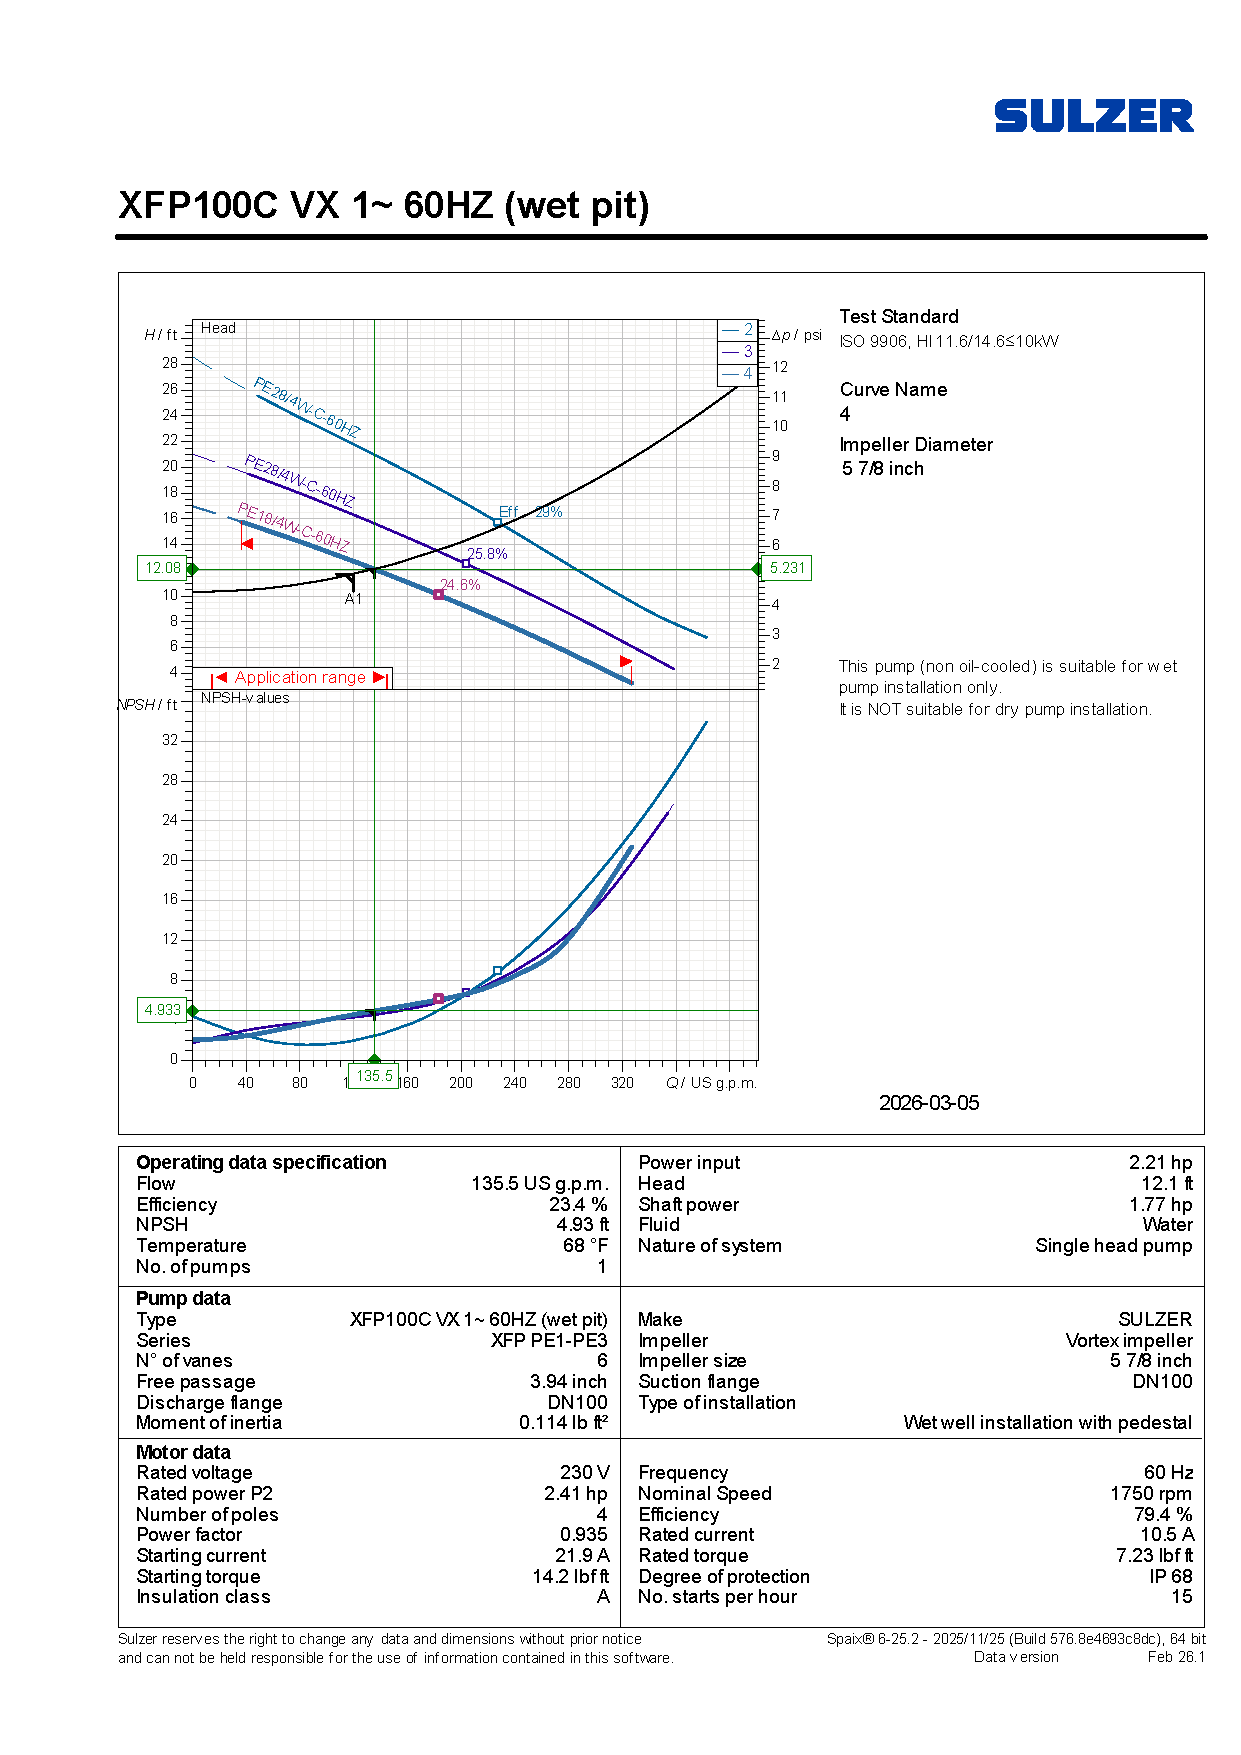
\includegraphics[
width=\textwidth,
trim={0.79in 4.3in 2.7in 2in},
clip
]{sulzer_xfp100c_curve.pdf}
\caption{Pump performance curve showing intersection with the system curve and selected operating point for the Sulzer XFP100C VX pump.}
\label{fig:pump_curve_intersection}
\end{figure}

The intersection between the system curve and the manufacturer pump performance curve defines the operating point of the selected pump. As illustrated in Figure~\ref{fig:pump_curve_intersection}, the selected Sulzer pump produces $135.5~\text{gpm}$ at a head of $12.08~\text{ft}$, which aligns with the hydraulic requirements of the system. This intersection confirms that the selected pump can deliver the required discharge while overcoming the calculated system head losses. The motor model at this point is PE 18/4W.

The performance data corresponding to the selected operating point are summarized in Table~\ref{tab:pump_operating_point}.

\begin{table}[H]
\centering
\caption{Selected Pump Operating Conditions}
\label{tab:pump_operating_point}
\begin{tabular}{lc}
\toprule
\textbf{Parameter} & \textbf{Value} \\
\midrule
Flow & 120 gpm (system design point) \\
Pump operating flow & 135.5 gpm \\
Total Dynamic Head & 12.08 ft \\
Hydraulic efficiency & 23.38 \% \\
Shaft power & 1.765 hp \\
\bottomrule
\end{tabular}
\end{table}

According to the manufacturer performance data, the selected pump operates at $135.5~\text{gpm}$ and $12.08~\text{ft}$ of head, with a hydraulic efficiency of $23.38~\%$ and a shaft power requirement of $1.765~\text{hp}$. The pump utilizes a vortex impeller that allows the passage of wastewater containing suspended solids and fibrous materials, which is a typical requirement for municipal wastewater pumping systems \cite{MetcalfEddy_Wastewater_2014}. The unit is designed for wet well installation and is equipped with an IE3 premium-efficiency motor operating at $1772~\text{rpm}$ \cite{Sulzer_PumpCatalog_2024}.

These performance parameters confirm that the selected Sulzer pump satisfies the hydraulic requirements of the lift station and provides adequate solids-handling capability for wastewater service. The motor power requirement identified from the manufacturer performance data will be used in the following section to determine the electrical and power requirements of the pump station.


% -------------------------------------------------
% 4.4 Pump Power Requirement and Motor Configuration
% -------------------------------------------------
\subsection{Pump Power Requirement and Motor Configuration}

The power requirement for the selected pump was obtained directly from the manufacturer performance data provided through the Sulzer ABSEL pump selection tool. At the selected operating condition, the Sulzer XFP100C VX 1$\sim$ (wet pit) pump delivers $135.5~\text{gpm}$ at $12.08~\text{ft}$ of head with a shaft power requirement of $1.765~\text{hp}$ and a motor output of $2.414~\text{hp}$. These values are taken from the manufacturer pump performance curves and therefore represent the required power for the selected operating point of the system \cite{Sulzer_ABSEL,Sulzer_PumpCatalog_2024}. The pump is equipped with a Sulzer PE18/4W motor operating at $230~\text{V}$, $60~\text{Hz}$, and $1772~\text{rpm}$, which defines the electrical capacity required for the lift station pump.

The selected unit utilizes a vortex impeller, which is commonly used in wastewater pumping applications. Jensen explains that vortex impellers are positioned toward the rear of the pump casing so that the rotating impeller generates a forced vortex that transports solids through the pump without requiring them to pass directly through the impeller vanes. This configuration improves reliability in sewage applications by allowing the passage of fibrous material and suspended solids while reducing the likelihood of clogging \cite{Jensen_PumpStationDesignGuidelines_2012}. For the Colebrooke Subdivision lift station, the vortex impeller was selected because reliability and solids-handling capability are critical for residential wastewater service.

The internal configuration of a typical submersible wastewater pump is illustrated in Figure~\ref{fig:submersible_pump_components}. The diagram shows the major mechanical elements including the motor assembly, shaft, bearings, mechanical seals, oil chamber, and impeller. These components work together to transmit motor power to the impeller while protecting the motor and bearings from wastewater intrusion.

\begin{figure}[H]
\centering
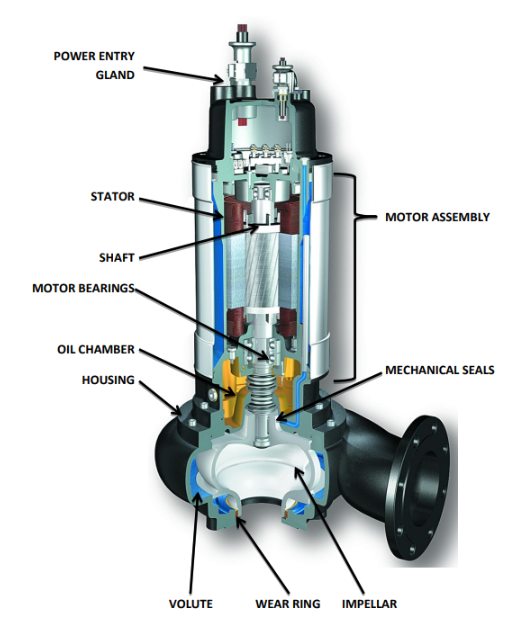
\includegraphics[width=0.7\textwidth]{components_of_a_pump.png}
\caption{Internal components of a submersible wastewater pump. Courtesy: Homa Pumps. \cite{HOMA_HazenWilliams_1998}}
\label{fig:submersible_pump_components}
\end{figure}

The selected pump incorporates a sealed submersible motor with an oil chamber and dual mechanical seals, which protect the motor and bearings from liquid intrusion during operation. Oil-filled submersible motors are commonly used in wastewater pumps because the oil improves heat transfer and provides continuous lubrication for internal components. The pump assembly also includes radial and axial load-supporting bearings designed by the manufacturer to withstand the hydraulic loads generated during pumping operation \cite{Jensen_PumpStationDesignGuidelines_2012}. These features ensure reliable operation of the pump under continuous wastewater service conditions.
